\documentclass[a4paper]{article}
\usepackage{graphicx}
\usepackage{amsmath}
\usepackage{listings}
\usepackage{float}
\usepackage{hyperref} 
\renewcommand{\thesection}{\arabic{section}}

\author{Grupo: \\
Mateus Ribeiro - 555225\\
Hubert Luz - 552798 \\
Vinícius Lôbo - 554036\\
}
\title{Filtro FIR Passa-Baixa para Limpeza de Áudio}
\begin{document}

\maketitle

\vspace{15mm}
\section{Introdução}
Os filtros FIR (Finite Impulse Response) são utilizados em processamento de sinais devido à sua estabilidade e resposta de fase linear. 
Um filtro FIR passa-baixa permite a passagem de frequências abaixo de uma frequência de corte específica, atenuando as frequências acima dessa frequência. 
Eles são utilizados em remoção de ruídos de alta frequência em sinais de áudio, pré-processamento de sinais em 
sistemas de comunicação, dentre outras aplicações.

\section{Métodos}
Neste trabalho, implementamos um filtro FIR passa-baixa para limpar dois sinais de áudio, removendo ruídos de alta frequência. 
Utilizamos a linguagem de programação Python para criar, aplicar o filtro e visualizar os resultados.

\subsection{Análise dos Sinais Providos}
Primeiramente, realizamos a leitura dos arquivos .wav e os plotamos para vizualizar como o sinal estava tanto no domínio do tempo
quanto no domínio da frequência.

Para realizar o plot no domínio do tempo, pegamos o número de amostras de cada sinal para que pudéssemos calcular o tempo total dele, 
isso foi feito dividindo o número de amostras pela frequência, em seguida criamos um vetor de
tempo "t" que será usado para plotar o sinal no domínio do tempo.


Já para o plot no domínio na frequência, basta aplicarmos a transformada de fourier nos sinais usando
a função "fft()" e usar a função "fftfreq()" para pegar o vetor de frequências que correspondem aos componentes da transformada.
\begin{figure}[H]
    \centering
    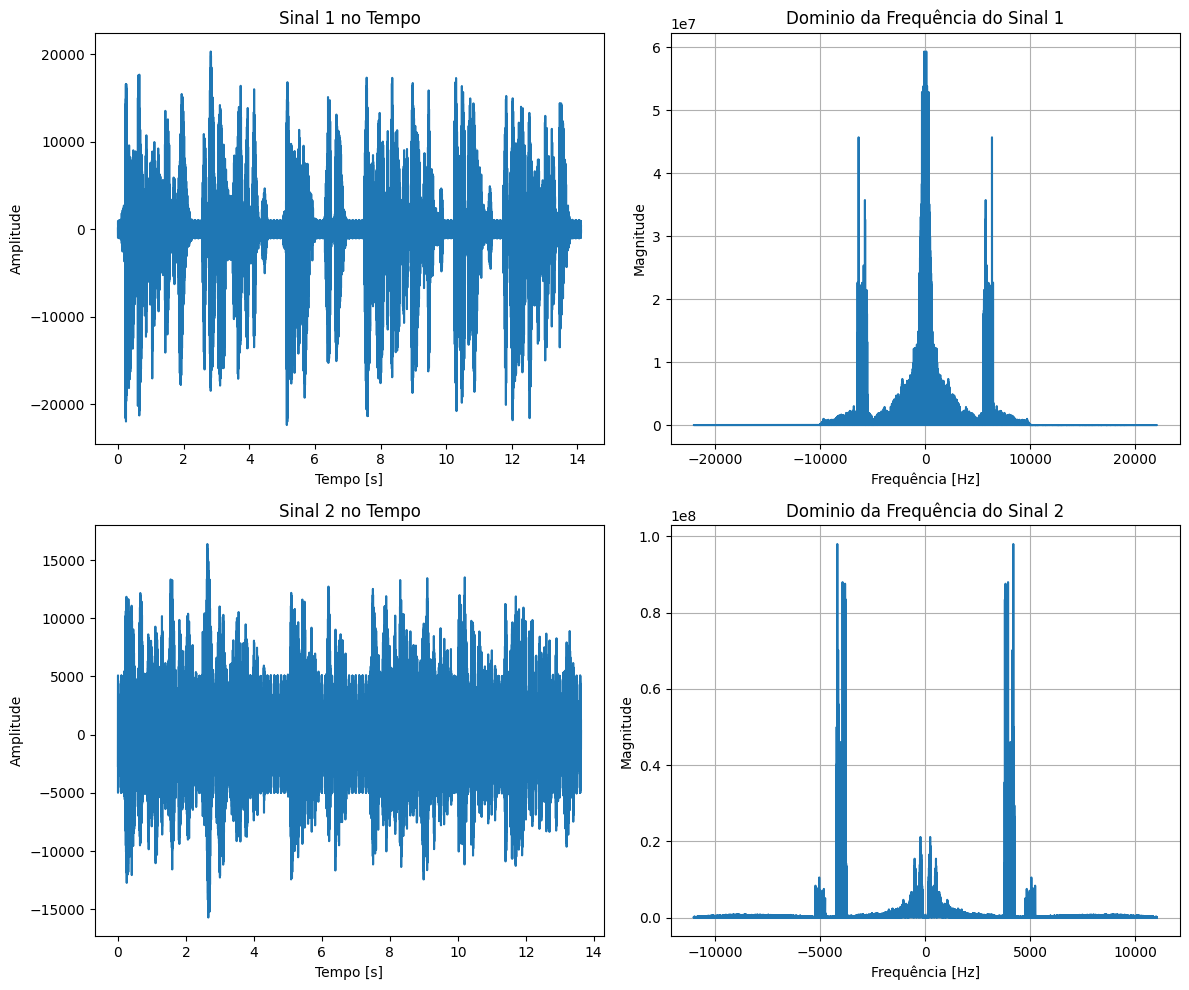
\includegraphics[width=0.8\textwidth]{../images/Plot_sinais.png}
    \caption{Sinal 1 Original no Tempo}
\end{figure}

Em seguida, utilizamos a função provida no material auxiliar para vizualizar o espectro de ambos os sinais.

\begin{lstlisting}[language=Python, caption=Função auxiliar]
    def spectrum(x_freq):
    # 
    # x_freq: vetor no dominio da frequencia, complexo
    #
    x_magnitude = np.abs(x_freq)
    # Normalizacao para o valor maximo ser 0dB
    x_magnitude /= np.max(x_magnitude)
    return 20*np.log10(x_magnitude)
    
\end{lstlisting}

Imagens obtidas para os espectros:

\begin{figure}[H]
    \centering
    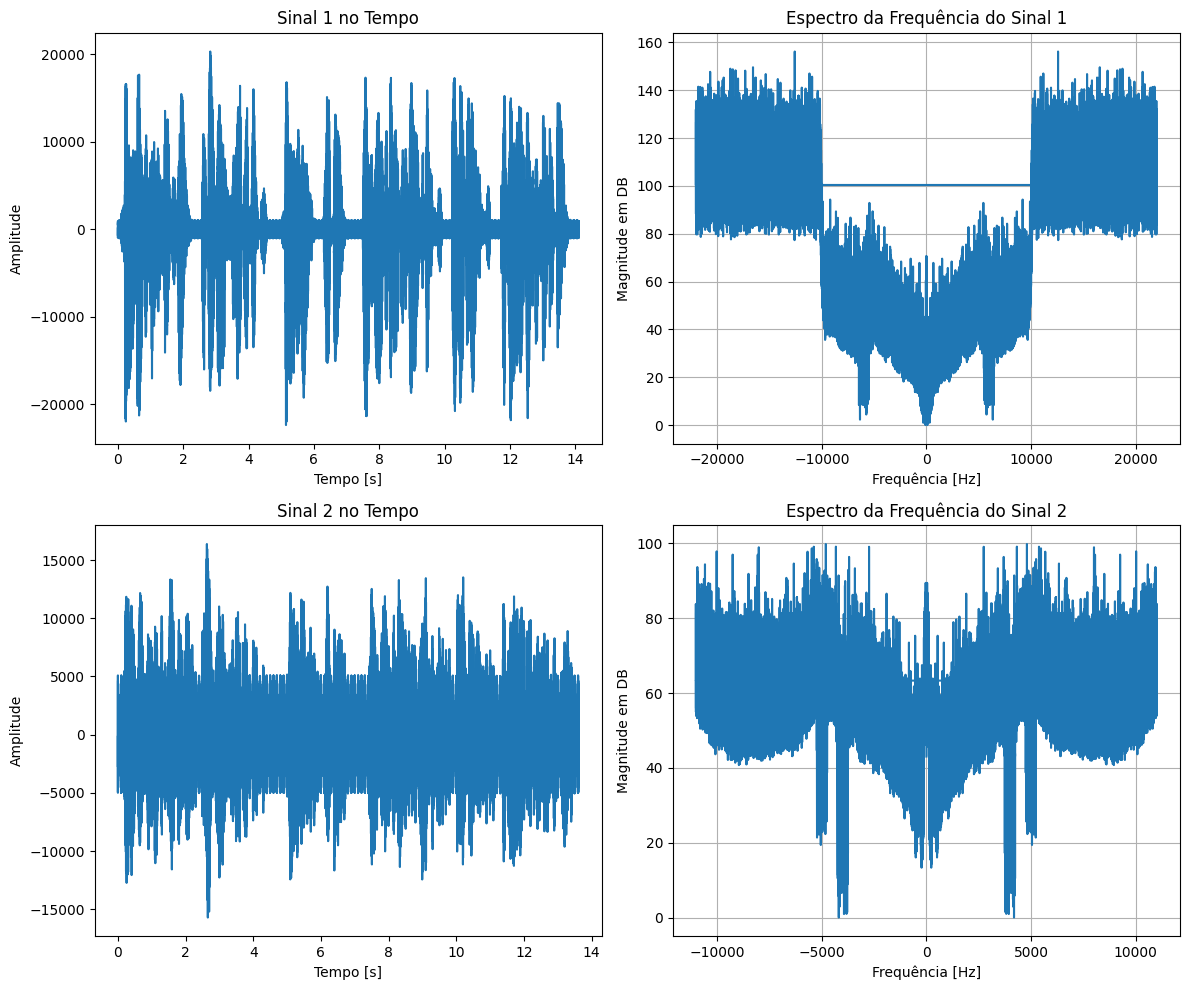
\includegraphics[width=0.8\textwidth]{../images/Plot_espectros.png}
    \caption{Sinal 1 Original no Tempo}
\end{figure}


Podemos vizualizar que:
\begin{itemize}
    \item Ao analisarmos o espectro do sinal 1, vemos que o ruído surge próximo aos 5000Hz, sendo assim, 
    utilizamos a frequencia de corte fc = 4800hz.
    \item De forma semelhante, o ruído no sinal 2 se mostra presente a partir dos 3600Hz, sendo assim, ajustamos a frequencia de corte fc = 3000Hz.
\end{itemize}

\subsection{Elaboração do Filtro}
Para o desenvolvimento do filtro, utilizamos como base teórica a seção 6.7.2 do livro 
"Oppenheim, A. V.; Willsky. A. S.; Nawabi, S. H. Sinais e Sistemas, 2a edição, Pearson,
2010." e o o capítulo 7 do livro "Digital Signal Processing Using MATLAB" do John G. Proakis, o qual foi recomendado 
em sala de aula durante o workshop para auxílio.

Para implementação, utilizamos o método de janelamento, o qual consiste em 
aplicar uma janela à uma função sinc para suavizar a transição da resposta em frequência 
e reduzir os efeitos do fenômeno de Gibbs. \footnote{\url{https://en.wikipedia.org/wiki/Gibbs_phenomenon}}

Em teoria, o filtro perfeito seria aplicar diretamente a resposta ao impulso da função sinc ao sinal:
\begin{equation}\label{eq:1}
    h[n] = 2 \cdot w_c \cdot sinc (2\cdot w_c \cdot n)
\end{equation}


Porém,a função sinc não é contínua em seus extremos e para resolver tal problema, utilizamos o método da janela de truncamento, onde escolhemos
"L" coeficientes para o filtro.

A janela escolhida foi a de Hamming, pois após pesquisarmos sobre, vimos que ela apresenta uma boa atenuação na banda de transição e atuanuação moderada
na banda de rejeição. A equação dela é:
\begin{equation}\label{eq:2}
    w[n] = 0.54 - 0.46 \cdot \cos({\frac{2\cdot\pi}{L-1}})
\end{equation}


Portanto, para implementar o filtro, devemos multiplicar a resposta ao impulso \ref{eq:1} por \ref{eq:2}

\begin{equation}\label{eq:3}
    h'[n] = h[n] \cdot w[n]
\end{equation}

É válido ressaltar que para a implementação, normalizamos a frequência com nyquist($f_n = \frac{SampleRate}{2}$), o que nos permite trabalhar com frequências entre 0 e 1 (independentes da taxa de amostragem), isso foi feito pois 
o design do filtro FIR se baseia na função sinc, a qual assume frequências normalizadas.
A resposta ao impulso do filtro:

\begin{figure}[H]
    \centering
    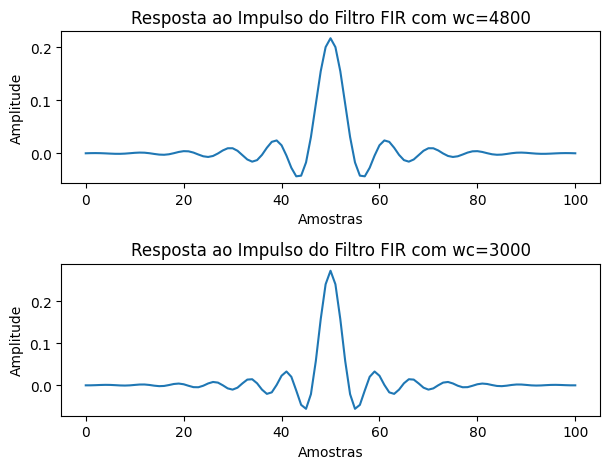
\includegraphics[width=0.8\textwidth]{../images/Plot_resposta_ao_impulso.png}
    \caption{Sinal 1 Original no Tempo}
\end{figure}

Para aplicar o filtro, iremos gozar da propriedade que diz que a convolução entre dois sinais no tempo corresponde ao produto de suas respectivas Transformadas de Fourier.

Ou seja, iremos calcular a fft do sinal e do filtro FIR, multiplicá-las e em seguida aplicar a ifft para retornar ao domínio do tempo. Um problema que encontramos é que o comprimento do filtro
é menor que o do sinal, por isso, tivemos que utilizar a técnica "zero-padding", ou seja, preencher com 0 o restante do vetor do filtro para igualar o tamanho com o do sinal.

\section{Resultados}
Os gráficos a seguir mostram os sinais de áudio originais e filtrados no domínio do tempo. 
Observa-se que os ruídos de alta frequência foram atenuados, resultando em sinais mais limpos e comprovando 
o funcionamento do filtro elaborado.

\begin{figure}[H]
    \centering
    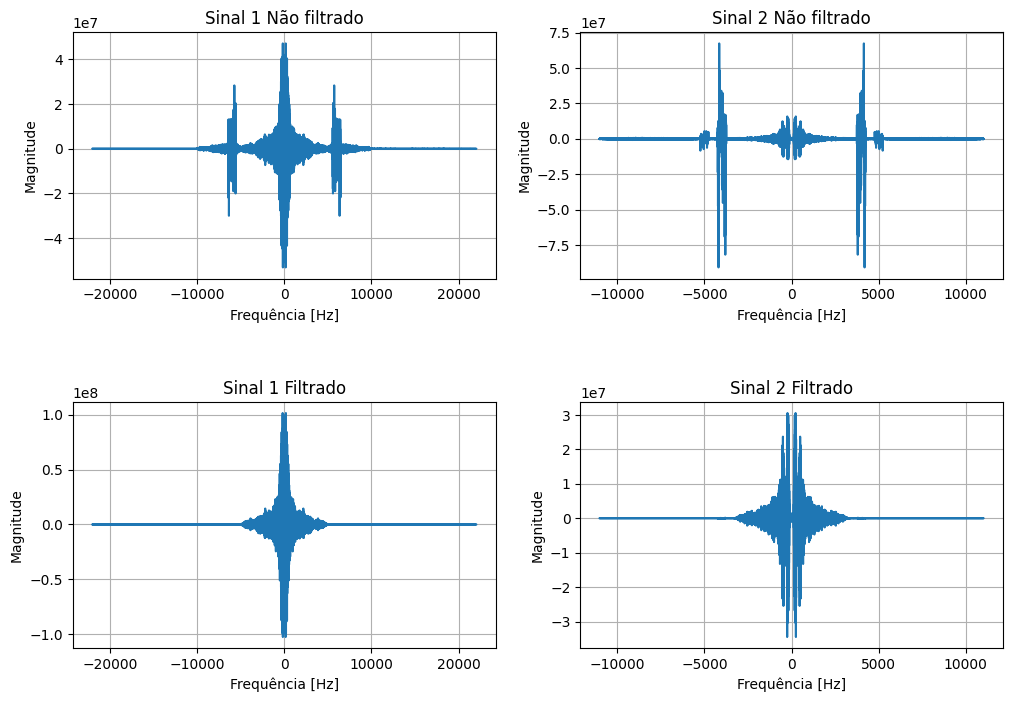
\includegraphics[width=0.8\textwidth]{../images/Plot_filtro.png}
    \caption{Sinal 1 Original no Tempo}
\end{figure}


\section{Conclusão}
Neste trabalho, foi possível colocar em prática os conhecimentos adiquiridos ao longo do semestre
na disciplina de Sinais e Sistemas na implementação um filtro FIR passa-baixa, vizando limpeza de sinais de áudio por meio
da remoção ruídos de alta frequência. Os sinais filtrados apresentaram uma redução 
significativa nos ruídos, resultando em uma qualidade de áudio melhorada.

\end{document}
